\documentclass[twoside]{book}

% Packages required by doxygen
\usepackage{fixltx2e}
\usepackage{calc}
\usepackage{doxygen}
\usepackage[export]{adjustbox} % also loads graphicx
\usepackage{graphicx}
\usepackage[utf8]{inputenc}
\usepackage{makeidx}
\usepackage{multicol}
\usepackage{multirow}
\PassOptionsToPackage{warn}{textcomp}
\usepackage{textcomp}
\usepackage[nointegrals]{wasysym}
\usepackage[table]{xcolor}

% Font selection
\usepackage[T1]{fontenc}
\usepackage[scaled=.90]{helvet}
\usepackage{courier}
\usepackage{amssymb}
\usepackage{sectsty}
\renewcommand{\familydefault}{\sfdefault}
\allsectionsfont{%
  \fontseries{bc}\selectfont%
  \color{darkgray}%
}
\renewcommand{\DoxyLabelFont}{%
  \fontseries{bc}\selectfont%
  \color{darkgray}%
}
\newcommand{\+}{\discretionary{\mbox{\scriptsize$\hookleftarrow$}}{}{}}

% Page & text layout
\usepackage{geometry}
\geometry{%
  a4paper,%
  top=2.5cm,%
  bottom=2.5cm,%
  left=2.5cm,%
  right=2.5cm%
}
\tolerance=750
\hfuzz=15pt
\hbadness=750
\setlength{\emergencystretch}{15pt}
\setlength{\parindent}{0cm}
\setlength{\parskip}{3ex plus 2ex minus 2ex}
\makeatletter
\renewcommand{\paragraph}{%
  \@startsection{paragraph}{4}{0ex}{-1.0ex}{1.0ex}{%
    \normalfont\normalsize\bfseries\SS@parafont%
  }%
}
\renewcommand{\subparagraph}{%
  \@startsection{subparagraph}{5}{0ex}{-1.0ex}{1.0ex}{%
    \normalfont\normalsize\bfseries\SS@subparafont%
  }%
}
\makeatother

% Headers & footers
\usepackage{fancyhdr}
\pagestyle{fancyplain}
\fancyhead[LE]{\fancyplain{}{\bfseries\thepage}}
\fancyhead[CE]{\fancyplain{}{}}
\fancyhead[RE]{\fancyplain{}{\bfseries\leftmark}}
\fancyhead[LO]{\fancyplain{}{\bfseries\rightmark}}
\fancyhead[CO]{\fancyplain{}{}}
\fancyhead[RO]{\fancyplain{}{\bfseries\thepage}}
\fancyfoot[LE]{\fancyplain{}{}}
\fancyfoot[CE]{\fancyplain{}{}}
\fancyfoot[RE]{\fancyplain{}{\bfseries\scriptsize Generated by Doxygen }}
\fancyfoot[LO]{\fancyplain{}{\bfseries\scriptsize Generated by Doxygen }}
\fancyfoot[CO]{\fancyplain{}{}}
\fancyfoot[RO]{\fancyplain{}{}}
\renewcommand{\footrulewidth}{0.4pt}
\renewcommand{\chaptermark}[1]{%
  \markboth{#1}{}%
}
\renewcommand{\sectionmark}[1]{%
  \markright{\thesection\ #1}%
}

% Indices & bibliography
\usepackage{natbib}
\usepackage[titles]{tocloft}
\setcounter{tocdepth}{3}
\setcounter{secnumdepth}{5}
\makeindex

% Hyperlinks (required, but should be loaded last)
\usepackage{ifpdf}
\ifpdf
  \usepackage[pdftex,pagebackref=true]{hyperref}
\else
  \usepackage[ps2pdf,pagebackref=true]{hyperref}
\fi
\hypersetup{%
  colorlinks=true,%
  linkcolor=blue,%
  citecolor=blue,%
  unicode%
}

% Custom commands
\newcommand{\clearemptydoublepage}{%
  \newpage{\pagestyle{empty}\cleardoublepage}%
}

\usepackage{caption}
\captionsetup{labelsep=space,justification=centering,font={bf},singlelinecheck=off,skip=4pt,position=top}

%===== C O N T E N T S =====

\begin{document}

% Titlepage & ToC
\hypersetup{pageanchor=false,
             bookmarksnumbered=true,
             pdfencoding=unicode
            }
\pagenumbering{alph}
\begin{titlepage}
\vspace*{7cm}
\begin{center}%
{\Large My Project }\\
\vspace*{1cm}
{\large Generated by Doxygen 1.8.12}\\
\end{center}
\end{titlepage}
\clearemptydoublepage
\pagenumbering{roman}
\tableofcontents
\clearemptydoublepage
\pagenumbering{arabic}
\hypersetup{pageanchor=true}

%--- Begin generated contents ---
\chapter{Hierarchical Index}
\section{Class Hierarchy}
This inheritance list is sorted roughly, but not completely, alphabetically\+:\begin{DoxyCompactList}
\item \contentsline{section}{Cell}{\pageref{classCell}}{}
\item \contentsline{section}{Coordinate}{\pageref{structCoordinate}}{}
\item \contentsline{section}{Map}{\pageref{classMap}}{}
\item \contentsline{section}{Map\+Editor\+Controller}{\pageref{classMapEditorController}}{}
\item \contentsline{section}{Map\+Validator}{\pageref{classMapValidator}}{}
\item \contentsline{section}{Map\+View}{\pageref{classMapView}}{}
\item Test\+Fixture\begin{DoxyCompactList}
\item \contentsline{section}{Map\+Test}{\pageref{classMapTest}}{}
\end{DoxyCompactList}
\end{DoxyCompactList}

\chapter{Class Index}
\section{Class List}
Here are the classes, structs, unions and interfaces with brief descriptions\+:\begin{DoxyCompactList}
\item\contentsline{section}{\hyperlink{classCell}{Cell} \\*Class to implement a cell }{\pageref{classCell}}{}
\item\contentsline{section}{\hyperlink{structCoordinate}{Coordinate} \\*Struct that represents a map coordinate }{\pageref{structCoordinate}}{}
\item\contentsline{section}{\hyperlink{classMap}{Map} \\*Class to implement the game map }{\pageref{classMap}}{}
\item\contentsline{section}{\hyperlink{classMapEditor}{Map\+Editor} \\*Class that implements the editor of the map }{\pageref{classMapEditor}}{}
\item\contentsline{section}{\hyperlink{classMapRenderer}{Map\+Renderer} \\*Class that implements logic to render map in command line interface }{\pageref{classMapRenderer}}{}
\item\contentsline{section}{\hyperlink{classMapTest}{Map\+Test} \\*Test Class for the \hyperlink{classMap}{Map} class }{\pageref{classMapTest}}{}
\item\contentsline{section}{\hyperlink{classMapValidator}{Map\+Validator} \\*Class that implements the logic for validating a map }{\pageref{classMapValidator}}{}
\end{DoxyCompactList}

\chapter{File Index}
\section{File List}
Here is a list of all documented files with brief descriptions\+:\begin{DoxyCompactList}
\item\contentsline{section}{src/controller/\hyperlink{MapEditorController_8h}{Map\+Editor\+Controller.\+h} \\*Header file containing class declaration for Map\+Editor.\+class }{\pageref{MapEditorController_8h}}{}
\item\contentsline{section}{src/entity/\hyperlink{Cell_8h}{Cell.\+h} \\*Header file containing class declaration for Cell.\+class }{\pageref{Cell_8h}}{}
\item\contentsline{section}{src/entity/\hyperlink{Map_8h}{Map.\+h} \\*Header file containing class declaration for Map.\+class and struct declaration for Coordinate.\+struct }{\pageref{Map_8h}}{}
\item\contentsline{section}{src/service/\hyperlink{MapValidator_8h}{Map\+Validator.\+h} \\*Header file containing class declaration for Map\+Validator.\+class }{\pageref{MapValidator_8h}}{}
\item\contentsline{section}{src/utils/\hyperlink{ArrayUtils_8h}{Array\+Utils.\+h} \\*Header file containing method declarations for useful 2D array manipulations }{\pageref{ArrayUtils_8h}}{}
\item\contentsline{section}{src/utils/\hyperlink{IOUtils_8h}{I\+O\+Utils.\+h} \\*Header file containing method declarations for useful IO operations }{\pageref{IOUtils_8h}}{}
\item\contentsline{section}{src/view/\hyperlink{MapView_8h}{Map\+View.\+h} \\*Header file containing class declaration for Map\+Renderer.\+class }{\pageref{MapView_8h}}{}
\item\contentsline{section}{tests/\hyperlink{MapTest_8cpp}{Map\+Test.\+cpp} \\*Implementation file for the \hyperlink{classMapTest}{Map\+Test} class }{\pageref{MapTest_8cpp}}{}
\end{DoxyCompactList}

\chapter{Class Documentation}
\hypertarget{classCell}{}\section{Cell Class Reference}
\label{classCell}\index{Cell@{Cell}}


Class to implement a cell.  




{\ttfamily \#include $<$Cell.\+h$>$}

\subsection*{Public Member Functions}
\begin{DoxyCompactItemize}
\item 
\hypertarget{classCell_aec0c2aa388ac3630108ab00cb5d0b723}{}\label{classCell_aec0c2aa388ac3630108ab00cb5d0b723} 
{\bfseries Cell} (char type)
\item 
\hypertarget{classCell_a92fc16bdcc26c2678122588898c5b84f}{}\label{classCell_a92fc16bdcc26c2678122588898c5b84f} 
char {\bfseries get\+Type} ()
\item 
\hypertarget{classCell_aec50a5f39f77075f0dea7e0abbea2827}{}\label{classCell_aec50a5f39f77075f0dea7e0abbea2827} 
void {\bfseries set\+Type} (char type)
\item 
\hypertarget{classCell_a730bbea4297eb0c7f2d943f75375f506}{}\label{classCell_a730bbea4297eb0c7f2d943f75375f506} 
char {\bfseries get\+Occupant} ()
\item 
\hypertarget{classCell_a782d9ced9f1345fafb5eb0feb04189a6}{}\label{classCell_a782d9ced9f1345fafb5eb0feb04189a6} 
void {\bfseries set\+Occupant} (char occupant)
\end{DoxyCompactItemize}
\subsection*{Static Public Attributes}
\begin{DoxyCompactItemize}
\item 
\hypertarget{classCell_aee89844377bf3c068f536d720059eb38}{}\label{classCell_aee89844377bf3c068f536d720059eb38} 
static const char {\bfseries T\+Y\+P\+E\+\_\+\+W\+A\+LL} = \textquotesingle{}w\textquotesingle{}
\item 
\hypertarget{classCell_a2817727832c0444ac1d133e26079bfac}{}\label{classCell_a2817727832c0444ac1d133e26079bfac} 
static const char {\bfseries T\+Y\+P\+E\+\_\+\+D\+O\+O\+R\+\_\+\+E\+N\+T\+RY} = \textquotesingle{}e\textquotesingle{}
\item 
\hypertarget{classCell_aecc7dd32172a9dcc250e425a56ecda3a}{}\label{classCell_aecc7dd32172a9dcc250e425a56ecda3a} 
static const char {\bfseries T\+Y\+P\+E\+\_\+\+D\+O\+O\+R\+\_\+\+E\+X\+IT} = \textquotesingle{}x\textquotesingle{}
\item 
\hypertarget{classCell_a61091404d91e4e167735507fd7a573dd}{}\label{classCell_a61091404d91e4e167735507fd7a573dd} 
static const char {\bfseries T\+Y\+P\+E\+\_\+\+F\+L\+O\+OR} = \textquotesingle{}f\textquotesingle{}
\item 
\hypertarget{classCell_a25529c63c082cbb3ca0bbc4248f764d5}{}\label{classCell_a25529c63c082cbb3ca0bbc4248f764d5} 
static const char {\bfseries O\+C\+C\+U\+P\+A\+N\+T\+\_\+\+C\+H\+E\+ST} = \textquotesingle{}c\textquotesingle{}
\item 
\hypertarget{classCell_a5d22265147c09d2e78464a7b709956dc}{}\label{classCell_a5d22265147c09d2e78464a7b709956dc} 
static const char {\bfseries O\+C\+C\+U\+P\+A\+N\+T\+\_\+\+O\+P\+P\+O\+N\+E\+NT} = \textquotesingle{}o\textquotesingle{}
\item 
\hypertarget{classCell_aea4173fcd295e2c4bfba5ed16e1e9a2c}{}\label{classCell_aea4173fcd295e2c4bfba5ed16e1e9a2c} 
static const char {\bfseries O\+C\+C\+U\+P\+A\+N\+T\+\_\+\+F\+R\+I\+E\+ND} = \textquotesingle{}r\textquotesingle{}
\item 
\hypertarget{classCell_accb7c7acaa1273831c44fb58c4846ca3}{}\label{classCell_accb7c7acaa1273831c44fb58c4846ca3} 
static const char {\bfseries O\+C\+C\+U\+P\+A\+N\+T\+\_\+\+E\+M\+P\+TY} = \textquotesingle{} \textquotesingle{}
\end{DoxyCompactItemize}


\subsection{Detailed Description}
Class to implement a cell. 

The documentation for this class was generated from the following files\+:\begin{DoxyCompactItemize}
\item 
src/entity/\hyperlink{Cell_8h}{Cell.\+h}\item 
src/entity/Cell.\+cpp\end{DoxyCompactItemize}

\hypertarget{structCoordinate}{}\section{Coordinate Struct Reference}
\label{structCoordinate}\index{Coordinate@{Coordinate}}


Struct that represents a map coordinate.  




{\ttfamily \#include $<$Map.\+h$>$}

\subsection*{Public Attributes}
\begin{DoxyCompactItemize}
\item 
\hypertarget{structCoordinate_a1731a846d76fa684b51477af2493a036}{}\label{structCoordinate_a1731a846d76fa684b51477af2493a036} 
int {\bfseries row}
\item 
\hypertarget{structCoordinate_aa98c59ced1ec817ab3fc64f8ce36e19a}{}\label{structCoordinate_aa98c59ced1ec817ab3fc64f8ce36e19a} 
int {\bfseries column}
\end{DoxyCompactItemize}


\subsection{Detailed Description}
Struct that represents a map coordinate. 

The documentation for this struct was generated from the following file\+:\begin{DoxyCompactItemize}
\item 
src/entity/\hyperlink{Map_8h}{Map.\+h}\end{DoxyCompactItemize}

\hypertarget{classMap}{}\section{Map Class Reference}
\label{classMap}\index{Map@{Map}}


Class to implement the game map.  




{\ttfamily \#include $<$Map.\+h$>$}

\subsection*{Public Member Functions}
\begin{DoxyCompactItemize}
\item 
\hypertarget{classMap_a3f402a90ac4a9e2c23f7d03baf593cd1}{}\label{classMap_a3f402a90ac4a9e2c23f7d03baf593cd1} 
{\bfseries Map} (int h, int w, \hyperlink{structCoordinate}{Coordinate} entry, \hyperlink{structCoordinate}{Coordinate} exit)
\item 
\hypertarget{classMap_a3bd3343daa6ffb33f400bff5d945a086}{}\label{classMap_a3bd3343daa6ffb33f400bff5d945a086} 
{\bfseries Map} (int h, int w)
\item 
\hypertarget{classMap_a2b09c8875af2efb711fc3a022e70427d}{}\label{classMap_a2b09c8875af2efb711fc3a022e70427d} 
int {\bfseries get\+Height} ()
\item 
\hypertarget{classMap_afd34d12227676b3cebeed9f5fae2508f}{}\label{classMap_afd34d12227676b3cebeed9f5fae2508f} 
int {\bfseries get\+Width} ()
\item 
\hypertarget{classMap_a02e6b6fa2643d26d51c8707b97c8271e}{}\label{classMap_a02e6b6fa2643d26d51c8707b97c8271e} 
\hyperlink{structCoordinate}{Coordinate} {\bfseries get\+Entry\+Door\+Coordinate} ()
\item 
\hypertarget{classMap_a08d73b6cc9dbb0447b550f1c7a9927be}{}\label{classMap_a08d73b6cc9dbb0447b550f1c7a9927be} 
\hyperlink{structCoordinate}{Coordinate} {\bfseries get\+Exit\+Door\+Coordinate} ()
\item 
\hypertarget{classMap_af2fc81e7365bae619097c4996845ed21}{}\label{classMap_af2fc81e7365bae619097c4996845ed21} 
void {\bfseries set\+Entry\+Door} (\hyperlink{structCoordinate}{Coordinate} entry\+Door)
\item 
\hypertarget{classMap_a86022f2db7773e6ea097605ad19f2569}{}\label{classMap_a86022f2db7773e6ea097605ad19f2569} 
void {\bfseries set\+Exit\+Door} (\hyperlink{structCoordinate}{Coordinate} exit\+Doors)
\item 
\hypertarget{classMap_ad06345e2fda83141117cf2260623b51f}{}\label{classMap_ad06345e2fda83141117cf2260623b51f} 
void {\bfseries init\+Doors} (\hyperlink{structCoordinate}{Coordinate} entry\+Door, \hyperlink{structCoordinate}{Coordinate} exit\+Door)
\item 
\hypertarget{classMap_ab8f7b8df6f5cfd061e37ceffefdad8c0}{}\label{classMap_ab8f7b8df6f5cfd061e37ceffefdad8c0} 
bool {\bfseries is\+Door} (int row, int column)
\item 
\hypertarget{classMap_ac00d085ca1148f6d8c282fbc85a38f71}{}\label{classMap_ac00d085ca1148f6d8c282fbc85a38f71} 
bool {\bfseries is\+Entry\+Door} (int row, int column)
\item 
\hypertarget{classMap_a6c85e5a96ec1e13c86b30a5054e2e260}{}\label{classMap_a6c85e5a96ec1e13c86b30a5054e2e260} 
bool {\bfseries is\+Exit\+Door} (int row, int column)
\item 
\hypertarget{classMap_a6dfb55208049862a7f66b177f6861878}{}\label{classMap_a6dfb55208049862a7f66b177f6861878} 
bool {\bfseries is\+Wall} (int row, int column)
\item 
\hypertarget{classMap_a6101fc8e14be52dba55b00584a8f0a1e}{}\label{classMap_a6101fc8e14be52dba55b00584a8f0a1e} 
bool {\bfseries is\+Floor} (int row, int column)
\item 
\hypertarget{classMap_aa088c6b9eb1ecfee30836e3046aee0db}{}\label{classMap_aa088c6b9eb1ecfee30836e3046aee0db} 
bool {\bfseries is\+Occupied} (int row, int column)
\item 
\hypertarget{classMap_ac303e5d0077a39a04855309df364d3fb}{}\label{classMap_ac303e5d0077a39a04855309df364d3fb} 
bool {\bfseries fill\+Cell} (int row, int column, char occupant)
\item 
\hypertarget{classMap_ad4279b4ede306ee50726ad391f35894c}{}\label{classMap_ad4279b4ede306ee50726ad391f35894c} 
char {\bfseries get\+Occupant} (int row, int column)
\item 
\hypertarget{classMap_a3be698445324a0d0e18b49d0730b9bea}{}\label{classMap_a3be698445324a0d0e18b49d0730b9bea} 
void {\bfseries render} ()
\item 
\hypertarget{classMap_a1e9b663a93c89e7775c66f5cb1b80573}{}\label{classMap_a1e9b663a93c89e7775c66f5cb1b80573} 
bool {\bfseries validate} ()
\item 
\hypertarget{classMap_a1b1fd198fc27787115aae3112e7bb5f1}{}\label{classMap_a1b1fd198fc27787115aae3112e7bb5f1} 
void {\bfseries set\+Cell\+Type} (int row, int column, char type)
\item 
\hypertarget{classMap_a6269d92c3dbdfddf220665beed78adae}{}\label{classMap_a6269d92c3dbdfddf220665beed78adae} 
bool {\bfseries is\+Inbound} (int row, int column)
\end{DoxyCompactItemize}


\subsection{Detailed Description}
Class to implement the game map. 

The documentation for this class was generated from the following files\+:\begin{DoxyCompactItemize}
\item 
src/entity/\hyperlink{Map_8h}{Map.\+h}\item 
src/entity/Map.\+cpp\end{DoxyCompactItemize}

\hypertarget{classMapEditorController}{}\section{Map\+Editor\+Controller Class Reference}
\label{classMapEditorController}\index{Map\+Editor\+Controller@{Map\+Editor\+Controller}}


Class that implements the editor of the map.  




{\ttfamily \#include $<$Map\+Editor\+Controller.\+h$>$}

\subsection*{Public Member Functions}
\begin{DoxyCompactItemize}
\item 
\hypertarget{classMapEditorController_a417086a846a4c2d470fd509f8701b736}{}\label{classMapEditorController_a417086a846a4c2d470fd509f8701b736} 
{\bfseries Map\+Editor\+Controller} (\hyperlink{classMap}{Map} $\ast$map)
\item 
\hypertarget{classMapEditorController_afe2d87da8000de0321d52103b75ddfc1}{}\label{classMapEditorController_afe2d87da8000de0321d52103b75ddfc1} 
void {\bfseries build\+Map} ()
\item 
\hypertarget{classMapEditorController_a55ea0d1c4f99a9d7903a66e4bb8a6dab}{}\label{classMapEditorController_a55ea0d1c4f99a9d7903a66e4bb8a6dab} 
\hyperlink{classMap}{Map} $\ast$ {\bfseries create\+Map} ()
\end{DoxyCompactItemize}


\subsection{Detailed Description}
Class that implements the editor of the map. 

The documentation for this class was generated from the following files\+:\begin{DoxyCompactItemize}
\item 
src/controller/\hyperlink{MapEditorController_8h}{Map\+Editor\+Controller.\+h}\item 
src/controller/Map\+Editor\+Controller.\+cpp\end{DoxyCompactItemize}

\hypertarget{classMapTest}{}\section{Map\+Test Class Reference}
\label{classMapTest}\index{Map\+Test@{Map\+Test}}


Test Class for the \hyperlink{classMap}{Map} class.  


Inheritance diagram for Map\+Test\+:\begin{figure}[H]
\begin{center}
\leavevmode
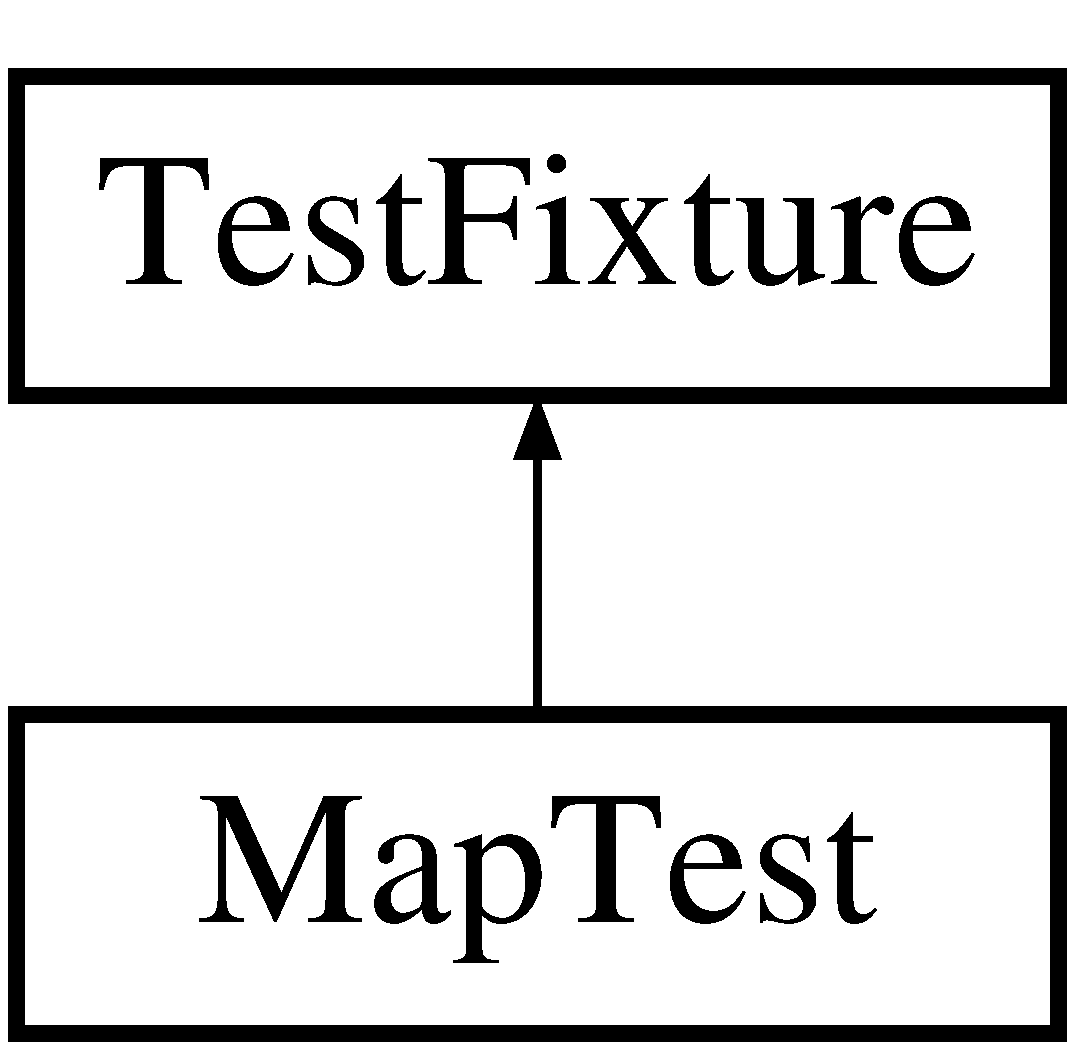
\includegraphics[height=2.000000cm]{classMapTest}
\end{center}
\end{figure}
\subsection*{Public Member Functions}
\begin{DoxyCompactItemize}
\item 
\hypertarget{classMapTest_a548501698e49e4de388482c502962cfd}{}\label{classMapTest_a548501698e49e4de388482c502962cfd} 
void \hyperlink{classMapTest_a548501698e49e4de388482c502962cfd}{set\+Up} ()
\begin{DoxyCompactList}\small\item\em method called before every test case in this test class \end{DoxyCompactList}\item 
\hypertarget{classMapTest_a1a75bd7462d39afc6f5039fa36252cca}{}\label{classMapTest_a1a75bd7462d39afc6f5039fa36252cca} 
void \hyperlink{classMapTest_a1a75bd7462d39afc6f5039fa36252cca}{tear\+Down} ()
\begin{DoxyCompactList}\small\item\em method called after every test case in this test class \end{DoxyCompactList}\end{DoxyCompactItemize}
\subsection*{Protected Member Functions}
\begin{DoxyCompactItemize}
\item 
void \hyperlink{classMapTest_a07e1aa96435351d15809b880ff7a7efb}{test\+Map\+Cell\+Filled} ()
\item 
void \hyperlink{classMapTest_a83bb3473f74089996c7f6bee8d59a97c}{test\+Map\+Cell\+Empty} ()
\item 
void \hyperlink{classMapTest_ae7a28d196c97101aa248a326af2a3f5b}{test\+Valid\+Path} ()
\item 
void \hyperlink{classMapTest_ad8823027d386c8d25f378d02adad120d}{test\+Invalid\+Path} ()
\item 
void \hyperlink{classMapTest_a577057c71af12efac9f1d6878bf85d01}{test\+Wall\+Cell} ()
\item 
void \hyperlink{classMapTest_a87e123f3f250492e1c444f0a3c8338b5}{test\+Is\+Door\+Cell} ()
\item 
void \hyperlink{classMapTest_a3e9eca91fbec359042f7287d378a3534}{tetst\+Fill\+Cell\+Failure} ()
\end{DoxyCompactItemize}


\subsection{Detailed Description}
Test Class for the \hyperlink{classMap}{Map} class. 

\subsection{Member Function Documentation}
\hypertarget{classMapTest_ad8823027d386c8d25f378d02adad120d}{}\label{classMapTest_ad8823027d386c8d25f378d02adad120d} 
\index{Map\+Test@{Map\+Test}!test\+Invalid\+Path@{test\+Invalid\+Path}}
\index{test\+Invalid\+Path@{test\+Invalid\+Path}!Map\+Test@{Map\+Test}}
\subsubsection{\texorpdfstring{test\+Invalid\+Path()}{testInvalidPath()}}
{\footnotesize\ttfamily void Map\+Test\+::test\+Invalid\+Path (\begin{DoxyParamCaption}{ }\end{DoxyParamCaption})\hspace{0.3cm}{\ttfamily [protected]}}

test method to test the validate\+Path() method of the \hyperlink{classMap}{Map} class Test Case\+: the returned value should be false if there is no valid path in the map Tested item\+: Map\+::validate\+Path() \hypertarget{classMapTest_a87e123f3f250492e1c444f0a3c8338b5}{}\label{classMapTest_a87e123f3f250492e1c444f0a3c8338b5} 
\index{Map\+Test@{Map\+Test}!test\+Is\+Door\+Cell@{test\+Is\+Door\+Cell}}
\index{test\+Is\+Door\+Cell@{test\+Is\+Door\+Cell}!Map\+Test@{Map\+Test}}
\subsubsection{\texorpdfstring{test\+Is\+Door\+Cell()}{testIsDoorCell()}}
{\footnotesize\ttfamily void Map\+Test\+::test\+Is\+Door\+Cell (\begin{DoxyParamCaption}{ }\end{DoxyParamCaption})\hspace{0.3cm}{\ttfamily [protected]}}

test method to test the is\+Wall() method of the \hyperlink{classMap}{Map} class Test Case\+: the returned value should be true if the cell is of type entry door or exit door Tested item\+: Map\+::is\+Door() \hypertarget{classMapTest_a83bb3473f74089996c7f6bee8d59a97c}{}\label{classMapTest_a83bb3473f74089996c7f6bee8d59a97c} 
\index{Map\+Test@{Map\+Test}!test\+Map\+Cell\+Empty@{test\+Map\+Cell\+Empty}}
\index{test\+Map\+Cell\+Empty@{test\+Map\+Cell\+Empty}!Map\+Test@{Map\+Test}}
\subsubsection{\texorpdfstring{test\+Map\+Cell\+Empty()}{testMapCellEmpty()}}
{\footnotesize\ttfamily void Map\+Test\+::test\+Map\+Cell\+Empty (\begin{DoxyParamCaption}{ }\end{DoxyParamCaption})\hspace{0.3cm}{\ttfamily [protected]}}

test method to test the is\+Occupied() method of the \hyperlink{classMap}{Map} class Test Case\+: the returned value should be true after emptying the cell Tested item\+: Map\+::is\+Occupied() \hypertarget{classMapTest_a07e1aa96435351d15809b880ff7a7efb}{}\label{classMapTest_a07e1aa96435351d15809b880ff7a7efb} 
\index{Map\+Test@{Map\+Test}!test\+Map\+Cell\+Filled@{test\+Map\+Cell\+Filled}}
\index{test\+Map\+Cell\+Filled@{test\+Map\+Cell\+Filled}!Map\+Test@{Map\+Test}}
\subsubsection{\texorpdfstring{test\+Map\+Cell\+Filled()}{testMapCellFilled()}}
{\footnotesize\ttfamily void Map\+Test\+::test\+Map\+Cell\+Filled (\begin{DoxyParamCaption}{ }\end{DoxyParamCaption})\hspace{0.3cm}{\ttfamily [protected]}}

test method to test the is\+Occupied() method of the \hyperlink{classMap}{Map} class Test Case\+: the returned value should be true after filling the cell Tested item\+: Map\+::is\+Occupied() \hypertarget{classMapTest_ae7a28d196c97101aa248a326af2a3f5b}{}\label{classMapTest_ae7a28d196c97101aa248a326af2a3f5b} 
\index{Map\+Test@{Map\+Test}!test\+Valid\+Path@{test\+Valid\+Path}}
\index{test\+Valid\+Path@{test\+Valid\+Path}!Map\+Test@{Map\+Test}}
\subsubsection{\texorpdfstring{test\+Valid\+Path()}{testValidPath()}}
{\footnotesize\ttfamily void Map\+Test\+::test\+Valid\+Path (\begin{DoxyParamCaption}{ }\end{DoxyParamCaption})\hspace{0.3cm}{\ttfamily [protected]}}

test method to test the validate\+Path() method of the \hyperlink{classMap}{Map} class Test Case\+: the returned value should be true if there is a valid path in the map Tested item\+: Map\+::validate\+Path() \hypertarget{classMapTest_a577057c71af12efac9f1d6878bf85d01}{}\label{classMapTest_a577057c71af12efac9f1d6878bf85d01} 
\index{Map\+Test@{Map\+Test}!test\+Wall\+Cell@{test\+Wall\+Cell}}
\index{test\+Wall\+Cell@{test\+Wall\+Cell}!Map\+Test@{Map\+Test}}
\subsubsection{\texorpdfstring{test\+Wall\+Cell()}{testWallCell()}}
{\footnotesize\ttfamily void Map\+Test\+::test\+Wall\+Cell (\begin{DoxyParamCaption}{ }\end{DoxyParamCaption})\hspace{0.3cm}{\ttfamily [protected]}}

test method to test the is\+Wall() method of the \hyperlink{classMap}{Map} class Test Case\+: the returned value should be true if the cell is of type wall Tested item\+: Map\+::is\+Wall() \hypertarget{classMapTest_a3e9eca91fbec359042f7287d378a3534}{}\label{classMapTest_a3e9eca91fbec359042f7287d378a3534} 
\index{Map\+Test@{Map\+Test}!tetst\+Fill\+Cell\+Failure@{tetst\+Fill\+Cell\+Failure}}
\index{tetst\+Fill\+Cell\+Failure@{tetst\+Fill\+Cell\+Failure}!Map\+Test@{Map\+Test}}
\subsubsection{\texorpdfstring{tetst\+Fill\+Cell\+Failure()}{tetstFillCellFailure()}}
{\footnotesize\ttfamily void Map\+Test\+::tetst\+Fill\+Cell\+Failure (\begin{DoxyParamCaption}{ }\end{DoxyParamCaption})\hspace{0.3cm}{\ttfamily [protected]}}

test method to test the fill\+Cell() method of the \hyperlink{classMap}{Map} class Test Case\+: the returned value should be true if an occupant was successfully added on the cell Tested item\+: Map\+::fill\+Cell() 

The documentation for this class was generated from the following file\+:\begin{DoxyCompactItemize}
\item 
tests/\hyperlink{MapTest_8cpp}{Map\+Test.\+cpp}\end{DoxyCompactItemize}

\hypertarget{classMapValidator}{}\section{Map\+Validator Class Reference}
\label{classMapValidator}\index{Map\+Validator@{Map\+Validator}}


Class that implements the logic for validating a map.  




{\ttfamily \#include $<$Map\+Validator.\+h$>$}

\subsection*{Public Member Functions}
\begin{DoxyCompactItemize}
\item 
\hypertarget{classMapValidator_a45fa5f33235b3e6de7666b6a5348c3a6}{}\label{classMapValidator_a45fa5f33235b3e6de7666b6a5348c3a6} 
{\bfseries Map\+Validator} (\hyperlink{classMap}{Map} $\ast$map)
\item 
\hypertarget{classMapValidator_a2066350c56590df7d109587034515f84}{}\label{classMapValidator_a2066350c56590df7d109587034515f84} 
bool {\bfseries validate\+Map} ()
\end{DoxyCompactItemize}


\subsection{Detailed Description}
Class that implements the logic for validating a map. 

The documentation for this class was generated from the following files\+:\begin{DoxyCompactItemize}
\item 
src/service/\hyperlink{MapValidator_8h}{Map\+Validator.\+h}\item 
src/service/Map\+Validator.\+cpp\end{DoxyCompactItemize}

\hypertarget{classMapView}{}\section{Map\+View Class Reference}
\label{classMapView}\index{Map\+View@{Map\+View}}


Class that implements logic to render map in command line interface.  




{\ttfamily \#include $<$Map\+View.\+h$>$}

\subsection*{Static Public Member Functions}
\begin{DoxyCompactItemize}
\item 
\hypertarget{classMapView_a6720017b6fc3902cf03ec6df87f363cd}{}\label{classMapView_a6720017b6fc3902cf03ec6df87f363cd} 
static void {\bfseries render\+Map} (\hyperlink{classMap}{Map} $\ast$map)
\end{DoxyCompactItemize}


\subsection{Detailed Description}
Class that implements logic to render map in command line interface. 

The documentation for this class was generated from the following files\+:\begin{DoxyCompactItemize}
\item 
src/view/\hyperlink{MapView_8h}{Map\+View.\+h}\item 
src/view/Map\+View.\+cpp\end{DoxyCompactItemize}

\chapter{File Documentation}
\hypertarget{MapEditorController_8h}{}\section{src/controller/\+Map\+Editor\+Controller.h File Reference}
\label{MapEditorController_8h}\index{src/controller/\+Map\+Editor\+Controller.\+h@{src/controller/\+Map\+Editor\+Controller.\+h}}


Header file containing class declaration for Map\+Editor.\+class.  


{\ttfamily \#include \char`\"{}../entity/\+Map.\+h\char`\"{}}\newline
\subsection*{Classes}
\begin{DoxyCompactItemize}
\item 
class \hyperlink{classMapEditorController}{Map\+Editor\+Controller}
\begin{DoxyCompactList}\small\item\em Class that implements the editor of the map. \end{DoxyCompactList}\end{DoxyCompactItemize}
\subsection*{Functions}
\begin{DoxyCompactItemize}
\item 
\hypertarget{MapEditorController_8h_a13f547b64c1a09dc6dac9c7d712fbbdc}{}\label{MapEditorController_8h_a13f547b64c1a09dc6dac9c7d712fbbdc} 
int {\bfseries read\+Map\+Dimension} (string message, int default\+Value, int min, int max)
\end{DoxyCompactItemize}


\subsection{Detailed Description}
Header file containing class declaration for Map\+Editor.\+class. 


\begin{DoxyEnumerate}
\item Game Rules\+: The code allows the player to create a map and populate it with the elements allowed by the game rules\+: friend character, enemy character, chest, door or wall. ~\newline
~\newline

\item Design\+: Controller class from the M\+VC pattern. It encapsulates all the logic to communicate with the user to create a map ~\newline
~\newline

\item Libraries\+: The implementation uses the string and regex libraries in order to parse the user input. The regex allows to validate the user provided a valid input 
\end{DoxyEnumerate}
\hypertarget{Cell_8h}{}\section{src/entity/\+Cell.h File Reference}
\label{Cell_8h}\index{src/entity/\+Cell.\+h@{src/entity/\+Cell.\+h}}


Header file containing class declaration for Cell.\+class.  


{\ttfamily \#include $<$iostream$>$}\newline
\subsection*{Classes}
\begin{DoxyCompactItemize}
\item 
class \hyperlink{classCell}{Cell}
\begin{DoxyCompactList}\small\item\em Class to implement a cell. \end{DoxyCompactList}\end{DoxyCompactItemize}
\subsection*{Functions}
\begin{DoxyCompactItemize}
\item 
\hypertarget{Cell_8h_ae136831e93b8454a5013821b11feecab}{}\label{Cell_8h_ae136831e93b8454a5013821b11feecab} 
void {\bfseries initialize\+Grid} (\hyperlink{classCell}{Cell} $\ast$$\ast$grid, int height, int width)
\end{DoxyCompactItemize}


\subsection{Detailed Description}
Header file containing class declaration for Cell.\+class. 


\begin{DoxyEnumerate}
\item Game Rules\+: A cell can be of type and/or contain game specific items\+: door, wall, friend or enemy character, and a chest ~\newline
~\newline

\item Design\+: Modlel class from the M\+VC pattern. Keeps the state of a cell by providing a type and an occupant ~\newline
~\newline

\item Libraries\+: No specific library used. 
\end{DoxyEnumerate}
\hypertarget{Map_8h}{}\section{src/entity/\+Map.h File Reference}
\label{Map_8h}\index{src/entity/\+Map.\+h@{src/entity/\+Map.\+h}}


Header file containing class declaration for Map.\+class and struct declaration for Coordinate.\+struct.  


{\ttfamily \#include $<$iostream$>$}\newline
{\ttfamily \#include \char`\"{}Cell.\+h\char`\"{}}\newline
\subsection*{Classes}
\begin{DoxyCompactItemize}
\item 
struct \hyperlink{structCoordinate}{Coordinate}
\begin{DoxyCompactList}\small\item\em Struct that represents a map coordinate. \end{DoxyCompactList}\item 
class \hyperlink{classMap}{Map}
\begin{DoxyCompactList}\small\item\em Class to implement the game map. \end{DoxyCompactList}\end{DoxyCompactItemize}


\subsection{Detailed Description}
Header file containing class declaration for Map.\+class and struct declaration for Coordinate.\+struct. 

No specific game rule enforced by the class except that a wall cannot be occupied. Design wise, the \hyperlink{classMap}{Map} class is a container of a 2D array of \hyperlink{classCell}{Cell} objects. The map does not use any specific library. 
\hypertarget{MapValidator_8h}{}\section{src/service/\+Map\+Validator.h File Reference}
\label{MapValidator_8h}\index{src/service/\+Map\+Validator.\+h@{src/service/\+Map\+Validator.\+h}}


Header file containing class declaration for Map\+Validator.\+class.  


{\ttfamily \#include \char`\"{}../entity/\+Map.\+h\char`\"{}}\newline
\subsection*{Classes}
\begin{DoxyCompactItemize}
\item 
class \hyperlink{classMapValidator}{Map\+Validator}
\begin{DoxyCompactList}\small\item\em Class that implements the logic for validating a map. \end{DoxyCompactList}\end{DoxyCompactItemize}


\subsection{Detailed Description}
Header file containing class declaration for Map\+Validator.\+class. 

No specific game rule enforced by the class. The class encapsulates the logic to validate a map. Concretely, it checks that each non-\/wall cell can be reached from the entry door of the map using a recursive function. The assumption is made that one can navigate from a cell to another in the following manner\+: up, down, right, left. To increase the performance of the algorithm, a cell not yet tested that was used in the path to reach the entry door while testing another cell is flagged as reachable. Consequently, this cell will be skipped when its turn comes for validation. No specific library is used. 
\hypertarget{ArrayUtils_8h}{}\section{src/utils/\+Array\+Utils.h File Reference}
\label{ArrayUtils_8h}\index{src/utils/\+Array\+Utils.\+h@{src/utils/\+Array\+Utils.\+h}}


Header file containing method declarations for useful 2D array manipulations.  


\subsection*{Functions}
\begin{DoxyCompactItemize}
\item 
\hypertarget{ArrayUtils_8h_a715a9580d392db4c43593d50d57aa0a0}{}\label{ArrayUtils_8h_a715a9580d392db4c43593d50d57aa0a0} 
void {\bfseries initialize2\+D\+Array} (bool $\ast$$\ast$grid, int height, int width)
\item 
\hypertarget{ArrayUtils_8h_a49d09d04dffade727d40ff823ab2c145}{}\label{ArrayUtils_8h_a49d09d04dffade727d40ff823ab2c145} 
void {\bfseries initialize2\+D\+Array} (int $\ast$$\ast$grid, int height, int width)
\item 
\hypertarget{ArrayUtils_8h_ae60e1dc4ec434fa691dca7ca37aefd90}{}\label{ArrayUtils_8h_ae60e1dc4ec434fa691dca7ca37aefd90} 
void {\bfseries reset2\+D\+Array} (bool $\ast$$\ast$grid, int height, int width)
\item 
\hypertarget{ArrayUtils_8h_a1f25dc67bedd5c4ccd2d23492409261d}{}\label{ArrayUtils_8h_a1f25dc67bedd5c4ccd2d23492409261d} 
void {\bfseries reset2\+D\+Array} (int $\ast$$\ast$grid, int height, int width)
\item 
\hypertarget{ArrayUtils_8h_a27471fd21a516c7704697e21f9148c93}{}\label{ArrayUtils_8h_a27471fd21a516c7704697e21f9148c93} 
void {\bfseries destroy2\+D\+Array} (bool $\ast$$\ast$grid, int height, int width)
\item 
\hypertarget{ArrayUtils_8h_a6e4ca4eb86ea18db5396ac0d10a7fcc6}{}\label{ArrayUtils_8h_a6e4ca4eb86ea18db5396ac0d10a7fcc6} 
void {\bfseries destroy2\+D\+Array} (int $\ast$$\ast$grid, int height, int width)
\end{DoxyCompactItemize}


\subsection{Detailed Description}
Header file containing method declarations for useful 2D array manipulations. 


\begin{DoxyEnumerate}
\item Game Rules\+: No specific game rule enforced by the class. ~\newline
~\newline

\item Design\+: Helper class for 2D array initialization and destruction. ~\newline
~\newline

\item No specific library is used. 
\end{DoxyEnumerate}
\hypertarget{IOUtils_8h}{}\section{src/utils/\+I\+O\+Utils.h File Reference}
\label{IOUtils_8h}\index{src/utils/\+I\+O\+Utils.\+h@{src/utils/\+I\+O\+Utils.\+h}}


Header file containing method declarations for useful IO operations.  


{\ttfamily \#include $<$iostream$>$}\newline
\subsection*{Functions}
\begin{DoxyCompactItemize}
\item 
\hypertarget{IOUtils_8h_a2cc142b5d955ac22d1529e7cf15802c6}{}\label{IOUtils_8h_a2cc142b5d955ac22d1529e7cf15802c6} 
bool {\bfseries read\+Yes\+No\+Input} (string prompt, bool default\+Ans)
\item 
\hypertarget{IOUtils_8h_afcbfc23eecc387ce3eabfa5a632eb403}{}\label{IOUtils_8h_afcbfc23eecc387ce3eabfa5a632eb403} 
string {\bfseries read\+String\+Input} (string prompt, string default\+Ans)
\item 
\hypertarget{IOUtils_8h_af69d86742da4f15ea813eb4ecdabf7d8}{}\label{IOUtils_8h_af69d86742da4f15ea813eb4ecdabf7d8} 
int {\bfseries read\+Integer\+Input} (string prompt, int default\+Ans)
\item 
\hypertarget{IOUtils_8h_a7a6849957d13fc5681327c2fc666b862}{}\label{IOUtils_8h_a7a6849957d13fc5681327c2fc666b862} 
double {\bfseries read\+Double\+Input} (string prompt, double default\+Ans)
\end{DoxyCompactItemize}


\subsection{Detailed Description}
Header file containing method declarations for useful IO operations. 


\begin{DoxyEnumerate}
\item Game Rules\+: No specific game rule enforced by the class. ~\newline
~\newline

\item Design\+: Provides method that encapsulate command line user input validation ~\newline
~\newline

\item Libraries\+: Uses the string std library to perform conversion from string to numbers 
\end{DoxyEnumerate}
\hypertarget{MapView_8h}{}\section{src/view/\+Map\+View.h File Reference}
\label{MapView_8h}\index{src/view/\+Map\+View.\+h@{src/view/\+Map\+View.\+h}}


Header file containing class declaration for Map\+Renderer.\+class.  


{\ttfamily \#include \char`\"{}../entity/\+Cell.\+h\char`\"{}}\newline
{\ttfamily \#include \char`\"{}../entity/\+Map.\+h\char`\"{}}\newline
\subsection*{Classes}
\begin{DoxyCompactItemize}
\item 
class \hyperlink{classMapView}{Map\+View}
\begin{DoxyCompactList}\small\item\em Class that implements logic to render map in command line interface. \end{DoxyCompactList}\end{DoxyCompactItemize}


\subsection{Detailed Description}
Header file containing class declaration for Map\+Renderer.\+class. 


\begin{DoxyEnumerate}
\item Game Rules\+: No specific game rule enforced by the class. ~\newline
~\newline

\item Design\+: View of the M\+VC pattern. Implements a Command Line Interface View of the \hyperlink{classMap}{Map}. ~\newline
~\newline

\item Libraries\+: No specific library is used apart from the iostream in order to display the map on the console 
\end{DoxyEnumerate}
\hypertarget{MapTest_8cpp}{}\section{tests/\+Map\+Test.cpp File Reference}
\label{MapTest_8cpp}\index{tests/\+Map\+Test.\+cpp@{tests/\+Map\+Test.\+cpp}}


Implementation file for the \hyperlink{classMapTest}{Map\+Test} class.  


{\ttfamily \#include $<$cppunit/\+Test\+Case.\+h$>$}\newline
{\ttfamily \#include $<$cppunit/\+Test\+Fixture.\+h$>$}\newline
{\ttfamily \#include $<$cppunit/ui/text/\+Text\+Test\+Runner.\+h$>$}\newline
{\ttfamily \#include $<$cppunit/extensions/\+Helper\+Macros.\+h$>$}\newline
{\ttfamily \#include $<$cppunit/extensions/\+Test\+Factory\+Registry.\+h$>$}\newline
{\ttfamily \#include $<$cppunit/\+Test\+Result.\+h$>$}\newline
{\ttfamily \#include $<$cppunit/\+Test\+Result\+Collector.\+h$>$}\newline
{\ttfamily \#include $<$cppunit/\+Test\+Runner.\+h$>$}\newline
{\ttfamily \#include $<$cppunit/\+Brief\+Test\+Progress\+Listener.\+h$>$}\newline
{\ttfamily \#include $<$cppunit/\+Compiler\+Outputter.\+h$>$}\newline
{\ttfamily \#include $<$cppunit/\+Xml\+Outputter.\+h$>$}\newline
{\ttfamily \#include \char`\"{}../src/entity/\+Map.\+h\char`\"{}}\newline
\subsection*{Classes}
\begin{DoxyCompactItemize}
\item 
class \hyperlink{classMapTest}{Map\+Test}
\begin{DoxyCompactList}\small\item\em Test Class for the \hyperlink{classMap}{Map} class. \end{DoxyCompactList}\end{DoxyCompactItemize}
\subsection*{Functions}
\begin{DoxyCompactItemize}
\item 
\hypertarget{MapTest_8cpp_a2ee438416ab9ccaf888fb81ef8291165}{}\label{MapTest_8cpp_a2ee438416ab9ccaf888fb81ef8291165} 
\hyperlink{MapTest_8cpp_a2ee438416ab9ccaf888fb81ef8291165}{C\+P\+P\+U\+N\+I\+T\+\_\+\+T\+E\+S\+T\+\_\+\+S\+U\+I\+T\+E\+\_\+\+R\+E\+G\+I\+S\+T\+R\+A\+T\+I\+ON} (\hyperlink{classMapTest}{Map\+Test})
\begin{DoxyCompactList}\small\item\em cppunit registry creation \end{DoxyCompactList}\end{DoxyCompactItemize}


\subsection{Detailed Description}
Implementation file for the \hyperlink{classMapTest}{Map\+Test} class. 


%--- End generated contents ---

% Index
\backmatter
\newpage
\phantomsection
\clearemptydoublepage
\addcontentsline{toc}{chapter}{Index}
\printindex

\end{document}
